% !TEX program = xelatex
% =====================================================================
% 使用说明书主文档
%
% 这是"用户手册 / 使用说明书"，回答"软件怎么用"。
% 源码清单在另一份 source-code.tex，两份文档分开编译。
%
% 章节取舍（软著只要求提交设计说明书、使用说明书之一，任选其一即可）：
%   - 界面型软件（Web / 桌面）：留 1、2、4、5、6、7
%   - 命令行工具：留 1、2、3、5、6、7
%   - 两者都有：全部保留
% 用不到的章节把下面的 \input 行注释掉即可，不要留空节。
% 每章写什么、哪些必写，见对应子文件顶部的注释。
% =====================================================================
\documentclass[
class = book,
zihao = -4,
font = noto,
paper = a4paper,
openany
]{easybook}

% !TEX program = xelatex
% 全局配置：只改本文件的软件名、版本号和字体，其余章节会自动引用。
% ============================================================

% Document info —— 改成你自己的软件信息
\newcommand{\Name}{DemoTool}
\newcommand{\NameCN}{轻量数据整理工具}
\newcommand{\FullName}{Lightweight Data Cleaning Toolkit}
\newcommand{\Version}{V1.0}
\newcommand{\Header}{\NameCN}

% 西文字体：正文 Times New Roman，无衬线 Arial，代码 DejaVu Sans Mono。
% 中文字体由 easybook.cls / ctex 管理，常用选项：font = noto 或 font = windows。
\newcommand{\ManualRomanFont}{Times New Roman}
\newcommand{\ManualSansFont}{Arial}
\newcommand{\ManualMonoFont}{DejaVu Sans Mono}
\AtBeginDocument{%
  \setmainfont{\ManualRomanFont}%
  \setsansfont{\ManualSansFont}%
  \setmonofont{\ManualMonoFont}%
}

% 代码框外观开关：手册用 decorated（默认带边框底色），源程序文档在
% source-code.tex 里改为 plain（纯白底无边框）。一般无需改这里。
\providecommand{\CodeBlockStyle}{decorated}
\newcommand{\PlainCodeBlockStyle}{plain}
\ifx\CodeBlockStyle\PlainCodeBlockStyle
  \lstdefinestyle{blockstyle}{
    style=basecode,
    basicstyle=\ttfamily\footnotesize,
    numbers=none,
    xleftmargin=1em,
    framexleftmargin=0pt,
    backgroundcolor={},
    frame=none
  }
  \lstdefinestyle{codestyle}{
    style=basecode,
    basicstyle=\ttfamily\scriptsize,
    numbers=none,
    numbersep=10pt,
    numberstyle=\tiny\color{codegray},
    xleftmargin=1em,
    framexleftmargin=0pt,
    backgroundcolor={},
    frame=none
  }
\fi

\usepackage{tikz}
\usetikzlibrary{positioning, arrows.meta, calc, fit}

\usepackage{zhlipsum,bicaption,tcolorbox}
\usepackage{longtable}
\usepackage{booktabs}
\usepackage{array}
\usepackage{ragged2e}
\usepackage{multirow}
\usepackage{float}
\usepackage[section]{placeins}
\usepackage[version=4]{mhchem}

% 定宽表格列：左对齐且禁止英文单词在单元格中断词。
\newcolumntype{L}[1]{>{\RaggedRight\arraybackslash\hyphenpenalty=10000\exhyphenpenalty=10000}p{#1}}

% 列表符号和正文一起缩进。
\setlist[itemize,1]{leftmargin=*, labelindent=2em, itemsep=2pt, topsep=4pt, parsep=0pt}
\setlist[enumerate,1]{leftmargin=*, labelindent=2em, itemsep=2pt, topsep=4pt, parsep=0pt}

% 行内长标识符在行尾按字符折行，避免把上一行中文撑开。
\newcommand{\cbr}[1]{\texttt{\seqsplit{#1}}}

% 放宽断行容忍度，避免长命令或路径把两端对齐的中文行撑开。
\tolerance=10000
\emergencystretch=3em
\hbadness=10000

\raggedbottom
\usepackage{seqsplit}
\usepackage{needspace}
\lstset{
	style=mystyle,
	escapeinside={(*@}{@*)} % 允许在代码中使用LaTeX命令
}

% 说明书版心：左右边距 2.54cm，减少长命令/路径/代码框换行。
\geometry{hmargin=2.54cm}

\begin{document}
	\title{\songti \NameCN \\ \Version \\ 使用说明}
	\date{\today}

	\frontmatter[roman]
	\maketitle
	\tableofcontents

	\mainmatter*

	% !TEX root = document.tex
% =====================================================================
% 第1章 引言 —— 所有软件类型都必写
%
% 写什么（按顺序）：
%   1. 编写目的：这份说明书是干什么的，一两句。
%   2. 软件简介与主要功能：软件解决什么问题、和已有工具比补了什么缺口、
%      功能清单（itemize）。这一段是全文最容易被写长的地方，控制在3段内。
%   3. 技术特点：自研的地方在哪，别写"性能优越"这类空话，写具体算法或机制。
%   4. 适用对象：谁用、需要什么前置知识，可顺带说明能力边界。
%   5. 第三方依赖声明：列许可证，明确"不对其主张著作权"。法律合规必写。
%
% 软著写作哲学：
%   - 第一章不要堆技术细节和代码，细节放第3/5章。
%   - 只写软件真实有的功能。示例命令、截图、输出都要能在源码里对应上。
%   - 不确定的背景就简略，正确比丰富重要。
%   - 软件名统一用 \Name / \NameCN / \Version，不要在正文里手写死。
% =====================================================================

\section{引言}
\label{sec:introduction}

\subsection{编写目的}
\label{ssec:intro_purpose}
本说明书用于说明"\Name"（版本号\Version）的开发背景、功能组成、实现方式和使用方法。文档内容对应当前版本的实际代码，用作安装、使用和软著登记材料中的技术说明。

\subsection{软件简介与主要功能}
\label{ssec:intro_summary}
"\Name"（以下简称\Name）面向结构化文本数据的整理场景，提供从文件读取、字段规范化、列筛选到完整性统计的一体化处理。使用者不必编写脚本，通过命令行子命令或浏览器界面即可完成常见的数据清洗任务。

\Name{}把"读取—清洗—统计—导出"串成一条固定流程，将常用操作收敛为若干条命令和一个可在浏览器中使用的页面，使同一套处理逻辑在自动脚本与交互式查看之间保持一致。

软件的主要功能包括：
\begin{itemize}
    \item 多种编码的CSV文件读取与写出
    \item 列名规范化与单元格空白清理
    \item 空行过滤与指定列筛选
    \item 逐列完整性统计与报告导出
    \item 命令行批量处理与浏览器交互操作两种使用方式
\end{itemize}

各项功能的实现方式见第五章，命令行用法见第三章，界面操作见第四章。

\subsection{技术特点}
\label{ssec:technical_features}
\Name{}的技术特点在于把清洗规则实现为可复用的纯函数，命令行与网页界面调用同一套核心模块，避免两种入口产生不同的处理结果。列名规范化采用确定性的映射与去重规则，同名列不会被覆盖；编码探测按候选列表逐个尝试，避免直接以默认编码打开非UTF-8文件。完整性统计以逐列为单位，缺失数与填充率由同一份数据计算得出。

\subsection{适用对象}
\label{ssec:intro_audience}
本软件适用于需要对表格型文本做批量整理的研究人员和数据工作者。使用命令行方式需具备基本的终端操作经验；使用浏览器界面只需会上传文件。软件面向结构化数据文件，不处理图像、音频等非文本格式，也不替代数据库系统。

\subsection{第三方依赖声明}
\label{ssec:third_party}
本软件自行实现文件读写、清洗规则、统计汇总、命令行解析与网页界面等逻辑。所依赖的第三方库著作权归各自作者所有，本软件仅按相应许可证使用，不对其主张著作权：
\begin{itemize}
    \item \textbf{Python}（PSF License）：核心开发语言。
    \item \textbf{Streamlit}（Apache-2.0）：浏览器交互界面。
\end{itemize}
上述许可证信息以各项目官方发布为准；使用前请核对对应版本的许可证条款。

	% !TEX root = document.tex
% =====================================================================
% 第2章 软件基本信息与安装 —— 所有软件类型都必写
%
% 写什么：
%   1. 软件基本信息表（三线表）：名称、版本、开发单位、完成日期、
%      运行平台、编程语言、依赖。必须和申请表 application.md 完全一致！
%   2. 系统要求：硬件（最低/推荐）+ 操作系统 + 核心依赖。
%   3. 获取与安装：安装命令、环境配置、启动方式。命令行和界面都写。
%
% 硬约束：
%   - 表中软件名、版本号必须与封面、申请表、源码页眉一致，审查会逐项核对。
%   - 界面截图上的名称必须与申请表上的软件名称一致。
%   - 每条软硬件环境描述控制在50字以内（申请表字数限制）。
%   - 表格用三线表并居中，长表格用 longtable。
% =====================================================================

\section{软件基本信息与安装配置}
\label{sec:installation}

\subsection{软件基本信息}
\label{ssec:software_info}
\begin{table}[H]
\centering
\begin{tabular}{ll}
\toprule
\textbf{项目} & \textbf{内容} \\
\midrule
软件名称 & \Name \\
软件简称 & \texttt{demo-tool}（命令行入口名） \\
版本号 & \Version{} \\
开发单位 & 示例单位（请替换为实际著作权人） \\
开发完成日期 & 2026年1月1日（请替换为实际日期） \\
运行平台 & Windows / Linux / macOS \\
编程语言 & Python 3.10+ \\
依赖库 & Streamlit \\
源代码网址 & \mbox{\url{https://example.org/your-repo}}（请替换） \\
\bottomrule
\end{tabular}
\caption{软件基本信息}
\label{tab:software_info}
\end{table}

表\ref{tab:software_info}中的软件名称、版本号与说明书封面及申请表保持一致。正式提交前，请把"示例单位""示例网址"等占位内容替换为真实信息。

\subsection{系统要求与环境准备}
\label{ssec:requirements}

\subsubsection{硬件要求}
最低配置：
\begin{itemize}
    \item CPU：2核及以上
    \item 内存：4~GB及以上
    \item 存储：100~MB可用空间
\end{itemize}
推荐配置：8核CPU、16~GB内存、SSD存储。

\subsubsection{操作系统支持}
\begin{itemize}
    \item Windows 10及以上
    \item Linux 主流发行版
    \item macOS 11及以上
\end{itemize}

\subsection{软件获取与安装}
\label{ssec:install}

\subsubsection{获取源码}
\begin{lstlisting}[language=bash,style=blockstyle]
git clone https://example.org/your-repo.git
cd your-repo
\end{lstlisting}
如无法使用Git，可在仓库页面下载源码压缩包后解压。

\subsubsection{创建运行环境}
\begin{lstlisting}[language=bash,style=blockstyle]
python -m venv .venv
source .venv/bin/activate        # Windows用 .venv\Scripts\activate
pip install -r requirements.txt
\end{lstlisting}

\subsubsection{启动方式}
命令行方式直接调用入口：
\begin{lstlisting}[language=bash,style=blockstyle]
python -m demo_tool --version
python -m demo_tool clean input.csv output.csv
\end{lstlisting}
浏览器界面方式启动服务后访问本地地址：
\begin{lstlisting}[language=bash,style=blockstyle]
streamlit run src/streamlit_app.py
\end{lstlisting}
启动后在浏览器打开\url{http://localhost:8501}即可使用界面。

	% !TEX root = document.tex
% =====================================================================
% 第3章 命令行使用方法 —— 命令行型软件的核心章，界面型软件可整章删掉
%
% 写什么：
%   1. 快速上手：一段可直接照抄的命令，从输入走到产出。放在最前面。
%   2. 命令清单：每个子命令一个小节，写清"做什么 + 命令样例 + 参数表 + 输出"。
%   3. 参数说明：逐个列参数含义，必需参数标注"必需"。
%   4. 输出文件：列出产物文件名和含义。
%   5. 典型流程：串起多个命令的完整例子。
%
% 排版约定：
%   - 命令块用 lstlisting，style=blockstyle，language填bash或python。
%   - 行内代码/参数名用 \lstinline|...|，下划线不用转义。
%   - 文字段落里的下划线用 \_，反斜杠用 \textbackslash。
%   - 命令行软件不写界面截图，截图留给第4章。
% =====================================================================

\section{命令行使用方法}
\label{sec:cli_usage}

本章说明\Name{}的命令行接口。所有命令通过\lstinline|python -m demo_tool|调用，后接子命令与参数。

\subsection{快速上手}
\label{ssec:cli_quickstart}
以下命令把一个CSV文件规范化后写出，并打印完整性报告：
\begin{lstlisting}[language=bash,style=blockstyle]
# 1. 查看版本，确认环境可用
python -m demo_tool --version

# 2. 清理列名与空白，去掉空行
python -m demo_tool clean raw.csv cleaned.csv

# 3. 只保留需要的列
python -m demo_tool select cleaned.csv selected.csv --columns name score

# 4. 生成完整性报告
python -m demo_tool report selected.csv --output report.csv
\end{lstlisting}
第4步结束后，\lstinline|selected.csv|为整理后的数据，\lstinline|report.csv|为逐列统计结果。

\subsection{命令清单}
\label{ssec:cli_commands}
软件提供三个子命令，分别用于清理、筛选和统计。

\subsubsection{clean}
\label{ssec:cli_clean}
规范化列名与单元格内容，按需要过滤空行：
\begin{lstlisting}[language=bash,style=blockstyle]
python -m demo_tool clean input.csv output.csv --keep-empty
\end{lstlisting}
参数说明：
\begin{itemize}
    \item \lstinline|input|（必需）：输入CSV文件路径。
    \item \lstinline|output|（必需）：输出CSV文件路径。
    \item \lstinline|--keep-empty|：保留空行；默认情况下空行被删除。
\end{itemize}
输出文件为UTF-8编码的CSV，列名统一为小写下划线形式，重复列名自动加序号后缀。

\subsubsection{select}
\label{ssec:cli_select}
按给定列名筛选并输出：
\begin{lstlisting}[language=bash,style=blockstyle]
python -m demo_tool select input.csv output.csv --columns name score
\end{lstlisting}
参数说明：
\begin{itemize}
    \item \lstinline|--columns|（必需）：要保留的列名，可跟多个。
\end{itemize}
列顺序与参数中给出的顺序一致；若指定了不存在的列，命令报错并列出未知列名。

\subsubsection{report}
\label{ssec:cli_report}
统计每行的总数、非空数与不同值个数：
\begin{lstlisting}[language=bash,style=blockstyle]
python -m demo_tool report input.csv --output report.csv
\end{lstlisting}
参数说明：
\begin{itemize}
    \item \lstinline|--output|：可选，把统计结果写成CSV；不指定时打印到终端。
\end{itemize}

\subsection{输出文件说明}
\label{ssec:cli_outputs}
\begin{table}[H]
\centering
\begin{tabular}{ll}
\toprule
\textbf{文件} & \textbf{含义} \\
\midrule
cleaned.csv & 列名规范化、空白清理后的数据 \\
selected.csv & 按指定列筛选后的数据 \\
report.csv & 逐列完整性统计结果 \\
\bottomrule
\end{tabular}
\caption{命令行输出文件}
\end{table}

\subsection{典型处理流程}
\label{ssec:cli_pipeline}
批量整理数据的完整顺序为：先用\lstinline|clean|统一格式，再用\lstinline|select|取需要的列，最后用\lstinline|report|检查缺失情况。三步的输入输出可以写成脚本循环，对多个文件重复执行。

	% !TEX root = document.tex
% =====================================================================
% 第4章 图形界面使用方法 —— 界面型软件的核心章，命令行软件可整章删掉
%
% 写什么（按顺序走一遍界面，像带人操作）：
%   1. 启动与登录：怎么打开、有没有登录。
%   2. 主界面：整体布局，放一张全屏截图。
%   3. 各功能模块：每个页面/按钮做什么，操作后发生什么，配截图。
%   4. 完整操作流程：从进入软件到拿到结果的连贯步骤。
%
% 截图的硬要求（审查重点）：
%   - 提供一张完整界面图建立整体印象，再用局部操作图说明关键步骤。
%   - 截图上的软件名称必须和申请表上的软件名称一致。
%   - 文字与截图要连贯：能看出页面怎么跳转、按了哪个按钮出现哪个界面。
%   - 图片放 images/ 目录，用 \includegraphics，宽度用 0.9\textwidth 之类。
%   - 图要清晰，太大就缩小，可用 subfigure 并排。
%
% 本章是示范文字，images/gui_home.png 为界面示意图，请替换为你的软件真实截图。完整界面图与局部操作图结合即可，不强制每张全屏。
% =====================================================================

\section{图形界面使用方法}
\label{sec:gui_usage}

本章以浏览器界面为例说明\Name{}的操作方式。界面与命令行共用同一套处理逻辑，两种方式的结果一致。

\subsection{启动与进入}
\label{ssec:gui_start}
按第\ref{sec:installation}章的命令启动服务后，在浏览器打开\url{http://localhost:8501}，进入软件首页。首页顶部显示软件名称，与申请表登记的名称一致。

\begin{figure}[!h]
\centering
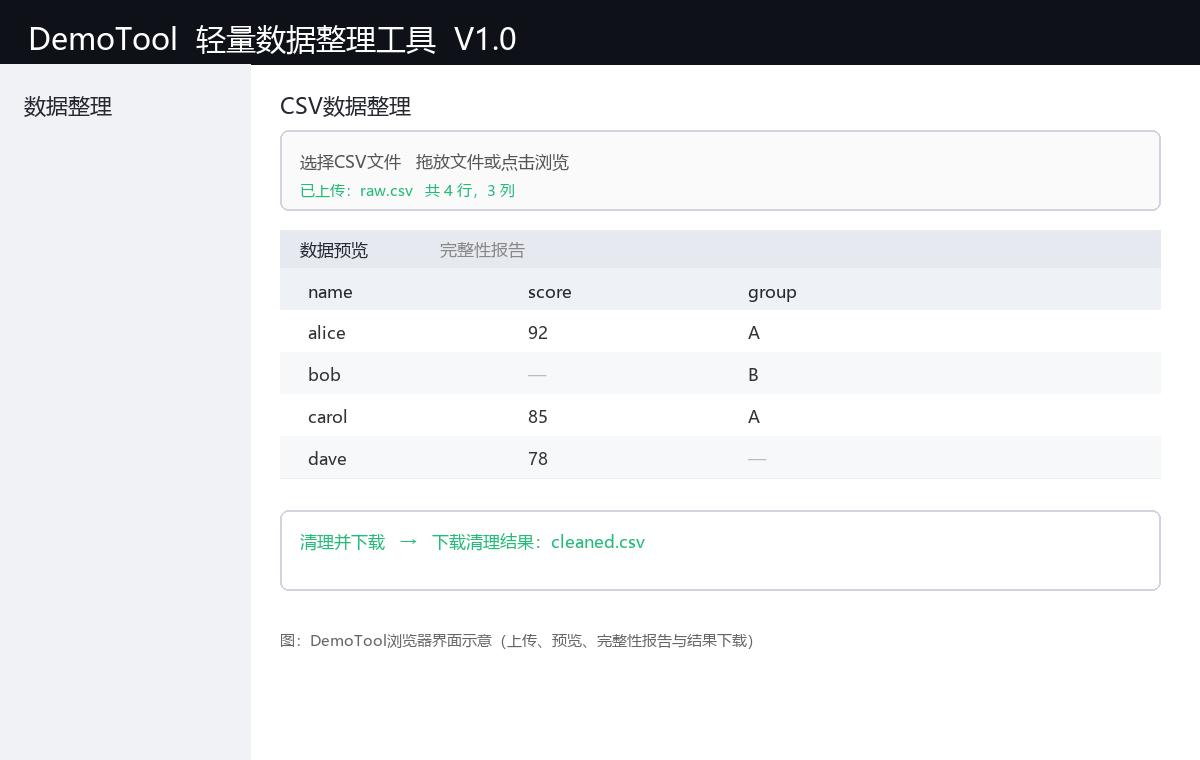
\includegraphics[width=0.9\textwidth]{images/gui_home.png}
\caption{\Name{}浏览器界面：上传、预览、报告与下载}
\label{fig:gui_home}
\end{figure}

\subsection{数据上传与预览}
\label{ssec:gui_upload}
在首页的"选择CSV文件"区域点击上传按钮，选取本地CSV文件。上传后页面显示数据行数与列数，并在"数据预览"标签页列出前20行。用户可在上传新文件替换当前数据。

上传与预览区域见前面\ref{fig:gui_home}的界面示意图。

\subsection{完整性报告}
\label{ssec:gui_report}
切换到"完整性报告"标签页，页面以表格形式列出每一列的总数、非空数、缺失数与不同值个数。缺失数由总数与非空数之差得到，用于判断哪些列需要先行清理。

\subsection{清理与下载}
\label{ssec:gui_clean}
点击页面下方的"清理并下载"按钮，软件对当前数据执行列名规范化、空白清理与空行过滤，生成\lstinline|cleaned.csv|。点击"下载清理结果"即可保存到本地。按钮所在界面见\ref{fig:gui_home}，操作结果在按钮下方给出下载入口。

\subsection{完整操作流程}
\label{ssec:gui_flow}
一次典型的界面操作按以下顺序进行：
\begin{enumerate}
    \item 启动服务并进入首页；
    \item 上传待整理的CSV文件；
    \item 在"数据预览"中确认文件内容与列结构；
    \item 在"完整性报告"中查看各列缺失情况；
    \item 点击"清理并下载"，保存结果文件。
\end{enumerate}
每一步对应的界面截图见前述各节。页面之间的跳转由标签页切换和按钮点击触发，截图与文字按顺序对应。

	% !TEX root = document.tex
% =====================================================================
% 第5章 软件架构与功能模块 —— 各类型都建议写，设计说明书的核心
%
% 软著哲学：审查人看这一章判断"这软件是不是真做了这些功能"。
% 写什么：
%   1. 架构图：一张模块图 + 一段文字说明分层。用 Mermaid 画，源在 materials/。
%   2. 模块说明：逐个模块写职责，和源码目录一一对应，别写空话。
%   3. 处理流程：编号列出主流程，对应到代码里的实际步骤。
%   4. 技术栈：列出语言、框架、库，和申请表一致。
%
% 注意：
%   - 架构图框内文字要少，太长就拆框，横向布局优先。
%   - 模块名、函数名要和真实源码一致，写完去代码里核对一遍。
%   - 软件名、术语全文统一。
% =====================================================================

\section{软件架构与功能模块}
\label{sec:architecture}

\subsection{总体架构}
\label{ssec:arch_overview}
\Name{}采用分层结构，由用户接口层、核心处理层与输入输出层组成。用户接口层提供命令行和浏览器两种入口；核心处理层实现清洗、筛选与统计；输入输出层负责文件的编码探测、读取与写出。两层入口调用同一套核心模块，保证结果一致。

\begin{figure}[htbp]
\centering
% 占位：用 materials/architecture.mmd 渲染后放到 images/ 下
% \includegraphics[width=0.9\textwidth]{images/architecture.png}
\caption{\Name{}软件架构与数据流示意图}
\label{fig:architecture}
\end{figure}

架构图对应的Mermaid源文件见\lstinline|materials/architecture.mmd|，可用Mermaid CLI渲染为PNG后放入\lstinline|images/|目录。

\subsection{模块说明}
\label{ssec:modules}
\begin{itemize}
    \item \textbf{io.py：} 文件输入输出。\lstinline|detect_encoding|按候选编码逐个尝试，避免直接用默认编码打开非UTF-8文件；\lstinline|read_rows|与\lstinline|write_rows|负责表格数据的读写。
    \item \textbf{core.py：} 核心清洗规则。\lstinline|normalize_header|把列名转为小写下划线形式并处理重名；\lstinline|trim_cells|清除单元格首尾空白；\lstinline|drop_empty_rows|过滤空行；\lstinline|select_columns|按指定列筛选并检查未知列。
    \item \textbf{report.py：} 统计汇总。\lstinline|summarize|逐列计算总数、非空数与不同值个数，\lstinline|ColumnSummary|提供缺失数与填充率。
    \item \textbf{cli.py：} 命令行入口。用\lstinline|argparse|定义\lstinline|clean|、\lstinline|select|、\lstinline|report|三个子命令，并分派到对应处理函数。
    \item \textbf{web.py：} 浏览器界面。基于Streamlit实现文件上传、数据预览、完整性报告与结果下载。
\end{itemize}

\subsection{处理流程}
\label{ssec:arch_flow}
一次完整的整理流程如下：
\begin{enumerate}
    \item 用户通过命令行或界面给出输入文件与处理参数；
    \item 输入输出层探测编码并读取数据为行列结构；
    \item 核心处理层按需执行列名规范化、空白清理、空行过滤或列筛选；
    \item 统计模块计算逐列完整性指标；
    \item 结果经输入输出层写出为CSV，或在界面中展示并提供下载。
\end{enumerate}

\subsection{技术栈}
\label{ssec:tech_stack}
\begin{itemize}
    \item \textbf{Python 3.10+：} 核心开发语言。
    \item \textbf{Streamlit：} 浏览器交互界面。
    \item \textbf{argparse：} 命令行参数解析。
\end{itemize}

	% !TEX root = document.tex
% =====================================================================
% 第6章 数据结构与文件说明 —— 有数据/文件/数据库的软件写，纯算法软件可删
%
% 写什么：
%   1. 输入输出文件格式：字段名、类型、含义，用三线表列成数据字典。
%   2. 内部数据结构：关键类或数据类有哪些字段。
%   3. 目录结构：源码目录树 + 每个目录/文件干什么。
%
% 注意：
%   - 表格用三线表居中，列名和类型要跟代码里的实际字段一致。
%   - 有数据库的软件在这一章写表结构、字段、主外键。
%   - 命令行和界面共用的数据格式只写一次，不要重复。
% =====================================================================

\section{数据结构与文件说明}
\label{sec:data_structure}

\subsection{输入文件格式}
\label{ssec:input_format}
软件接受UTF-8或GB18030编码的CSV文件，第一行为表头，其余每行一条记录。读取时会尝试候选编码列表中的每一种，直到能够完整解码。

\subsection{内部数据结构}
\label{ssec:internal_data}
读取后的数据表示为"表头列表 + 数据行列表"：表头是字符串列表，数据行是字符串列表的列表，二者下标一一对应。统计结果用\lstinline|ColumnSummary|数据类表示，字段含义如表\ref{tab:column_summary}所示。

\begin{table}[H]
\centering
\begin{tabular}{lll}
\toprule
\textbf{字段} & \textbf{类型} & \textbf{含义} \\
\midrule
name & str & 列名 \\
total & int & 该列记录总数 \\
filled & int & 非空单元格数 \\
distinct & int & 不同非空值个数 \\
\bottomrule
\end{tabular}
\caption{ColumnSummary字段说明}
\label{tab:column_summary}
\end{table}

\subsection{输出文件格式}
\label{ssec:output_format}
写出文件统一采用UTF-8带BOM编码的CSV，便于在表格软件中直接打开。报告文件包含\lstinline|column|、\lstinline|total|、\lstinline|filled|、\lstinline|distinct|、\lstinline|missing|五列。

\subsection{源码目录结构}
\label{ssec:dir_structure}
\begin{lstlisting}[language=bash,style=blockstyle]
src/demo_tool/
├── __init__.py      # 版本信息与包导出
├── io.py            # 编码探测与文件读写
├── core.py          # 清洗与筛选规则
├── report.py        # 完整性统计
├── cli.py           # 命令行入口
└── web.py           # 浏览器界面
\end{lstlisting}
各模块职责见第\ref{sec:architecture}章模块说明，函数实现见源程序文档。

	% !TEX root = document.tex
% =====================================================================
% 第7章 附录与修订记录 —— 可选，有第三方依赖或多次登记时写
%
% 写什么：
%   1. 第三方依赖许可证：和第一章声明呼应，列清单。
%   2. 版本历史：V1.0首次登记写"无历史版本"；高版本要说明新增功能，
%      并注明原软著登记号。
%   3. 参考资料：官方登记入口、法规名称。
%
% 注意：不要写"具体版本以封存环境为准"这类不该给审查人看的内部话。
% =====================================================================

\section{附录与修订记录}
\label{sec:appendix}

\subsection{主要第三方依赖许可证}
\label{ssec:license_list}
\begin{table}[H]
\centering
\begin{tabular}{ll}
\toprule
\textbf{依赖} & \textbf{许可证} \\
\midrule
Python & PSF License \\
Streamlit & Apache-2.0 \\
\bottomrule
\end{tabular}
\caption{主要第三方依赖及许可证}
\end{table}

\subsection{版本历史}
\label{ssec:version_history}
本版本为V1.0首次登记，无历史版本，无版本更新说明。若后续提交V2.0及以上版本，需在此说明相对低版本新增的功能，并注明原软件著作权登记号。

\subsection{参考资料}
\label{ssec:references}
\begin{itemize}
    \item 《计算机软件保护条例》
    \item 《计算机软件著作权登记办法》
    \item 中国版权保护中心：\url{https://www.ccopyright.com.cn}
\end{itemize}


	\backmatter
\end{document}
